\documentclass[a4paper,10pt]{article}
\usepackage[margin=1.4in]{geometry}
\usepackage[swedish]{babel}
\usepackage[utf8]{inputenc}
\usepackage{titlesec}
\usepackage{titling}
\usepackage{todonotes}



\setlength{\parskip}{1em}
\setlength{\parindent}{0pt}
\titlespacing{\section}{0pt}{\parskip}{-\parskip}
\titlespacing{\subsection}{0pt}{\parskip}{-\parskip}
\titlespacing{\subsubsection}{0pt}{\parskip}{-\parskip}
\titlespacing{\part}{0pt}{\parskip}{-\parskip}


\externaldocument[arkd-]{../Arkitekturdokument/arkitekturdokument}

\begin{document}
\def\ftitle{Testplan}
\def\fversion{1.0}
\begin{titlepage} % Suppresses displaying the page number on the title page and the subsequent page counts as page 1
	\newcommand{\HRule}{\rule{\linewidth}{0.5mm}} % Defines a new command for horizontal lines, change thickness here

	\center % Centre everything on the page

	%------------------------------------------------
	%	Headings
	%------------------------------------------------

	\textsc{\LARGE Linköpings universitet \\ \vspace{0.2em} Institutionen för datavetenskap }\\[2cm]

    \large\today

    \vspace{1cm}


	%------------------------------------------------
	%	Title
	%------------------------------------------------

	\HRule\\[0.4cm]

	{\huge\bfseries Schemaläggningsstöd för  kirurgi \vspace{.1em} \\ \ftitle }\\[0.4cm] % Title of your document

	\HRule\\[1cm]

	%------------------------------------------------
	%	Author(s)
	%------------------------------------------------

	\begin{minipage}{0.7\textwidth}
			\large
            \emph{Version: \fversion}
            \vspace{1em}

            \textbf{\\Adam Andersson, Niclas Byrsten, \\Björn Hvass, Henrik Lindström, \\Martin Persson, Christoffer Sjöbergsson, \\Tor Utterborn}


            \vspace{1em}

            Handledare: Jonas Wallgren

            Examinator: Kristian Sandahl
	\end{minipage}
	~

	%------------------------------------------------
	%	Logo
	%------------------------------------------------

	%\vfill\vfill
	%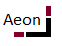
\includegraphics[width=0.2\textwidth]{../Templates/Aeon}\\[1cm] % Include a department/university logo - this will require the graphicx package

	%----------------------------------------------------------------------------------------

	\vfill % Push the date up 1/4 of the remaining page

\end{titlepage}


\section*{\begin{center}Projektidentitet\end{center}}
    \vspace{-2.5em}
    \begin{center}
        \begin{tabular}{|c c c|}
        \hline
        Namn & Roll & E-post \\
        \hline
        Adam Andersson& Teamleader & adam.e.a.andersson@gmail.com\\
        \hline
        Niclas Byrsten & Testansvarig & nicby889@student.liu.se\\
        \hline
        Björn Hvass & Konfigurationsansvarig & bjorn.hvass@gmail.com\\
        \hline
        Henrik Lindström & Utvecklingsledare & henli070@student.liu.se\\
        \hline
        Martin Persson & Arkitekturansvarig & marpe902@liu.student.se\\
        \hline
        Christoffer Sjöbersson & Analysansvarig & chrsj812@liu.student.se\\
        \hline
        Tor Utterborn & Dokument- \& Kvalitetsansvarig & tor.utterborn@gmail.com\\
        \hline
        \end{tabular}
    \end{center}

    \begin{center}
        \small
        \textbf{Kund}\\Region Östergötland, 581 91 Linköping.

        \textbf{Kontaktperson hos kund}\\
        Gunnar Nordqvist, IT-arkitekt, 010-1030698, Gunnar.Nordqvist@regionostergotland.se\\
        Erik Sundvall, Informationsarkitekt, 010-1036252, Erik.Sundvall@regionostergotland.se
    \end{center}

\vspace{9em}



\section*{\begin{center}Dokumentationshistorik\end{center}}
\begin{center}
 \begin{tabular}{|c c c c |}
 \hline
 Datum & händelse & iteration & version\\
 \hline
 2018-02-14 & Dokument skapas & 1 &  0.1\\
 \hline
  2018-02-19 & Konvertering till \textbf{\LaTeX} & 1 &  0.2\\
 \hline
   2018-02-19 & Version 1.0 färdigställd & 1 &  1.0\\
 \hline
\end{tabular}
\clearpage
\end{center}
\tableofcontents
\clearpage
\section{Inledning}
\label{sec:Inledning}
Det här dokumentet ska översiktligt beskriva de tester som kommer att genomföras under projektets gång.
\subsection{Syfte}
Syftet med denna kvalitetsplan är att beskriva de tekniker, aktiviteter och metoder som kommer att användas för att försäkra att en hög kvalitet hålls i projektet. Detta innebär att slutprodukten ska uppfylla alla krav, levereras i tid och hålla sig inom budgeten.
\subsection{Omfattning}
Syftet med denna testplan är att beskriva de tester som kommer att utföras. Målet är att dokumentera de tester som kommer att utföras för att säkerhetsställa systemets kvalitet som finns beskrivet i dokumentet Kvalitetsplan samt de krav som finns beskrivet i dokumentet Kravspec. Då Scrum är vald som arbetsmetodik så kommer det att vara tester på varje testnivå.
\subsection{Refererade dokument}
\label{sec:Refererade_dokument}
Följande interna dokument refereras till i detta dokument:
\begin{itemize}
	\item Projektplan
	\item Kravspecifikation
	\item Testplan
\end{itemize}
\subsection{Systemöversikt}
Se arkitekturdokumentet sektion \ref{arkd-sec:Systemskiss}.

\subsection{Testöversikt}
Denna del ger en översikt av testerna, vilken typ av tester, vilka resurser som kommer att användas, vilka som har ansvar för vilka test samt vilka verktyg och metoder som kommer att användas.

\subsubsection{Organisation}
Se sektion \ref{sec:Ansvarsomraden} Ansvarsområden.

\subsubsection{Testplanering}
Under iteration två ska pappersprototyper göras som en tidig design av gränssnittet och på så vis få feedback från både gruppen och kunden. Utöver den så kommer tester planeras fortlöpande genom projektet.

\subsubsection{Integrity level scheme}
\subsubsection{Resources summary}
\subsection{Ansvarsområden}
\label{sec:Ansvarsomraden}
Alla medlemmar har ansvar för de tester som utförs. Projektets testledare har övergripande ansvar för de tester som kommer att genomföras.
\subsection{Tools, techniques, methods, and metrics}
För verktyg se sektionen Verktyg i Kvalitetsplanen.
\section{Details of the Master Test Plan}
Den här sektionen beskriver processen, dokumentationen och rapporteringen för de tester som genomförs.
\subsection{Test processes including definition of test levels}
\begin{itemize}
	\item Pappersprototyp: Se sektion Pappersprototyper i Kvalitetsplan.\todo{mvoe to other place}
	\item Enhetstester: Ska genomföras regelbundet för att den kod som har skrivits fungerar. Den som skriver koden ska även utföra enhetstester regelbundet.
	\item Integrationstester: Om projektmedlemmar anser att ett delsystem är redo att integreras i systemet ska integrationstester utföras på detta delsystem.
	\item Systemtester: När alla delsystem anses uppfyllda ska dessa integreras och testas gentemot de krav som finns beskrivna i dokumentet Kravspec.
	\item Acceptanstester: För att säkerhetsställa att givna krav är uppfyllda ska kund testa systemet och ge återkoppling.
\end{itemize}

\subsubsection{Process: Management}
\subsubsection{Activity: Management of test effort}
\subsubsection{Process: Acquisition}
\subsubsection{Activity: Acquisition support test}
\subsubsection{Process: Supply}

...

\end{document}
